\chapter[Resultados obtidos]{Resultados obtidos}

O desenvolvimento do Traveller foi, desde seu início, fortemente testado por uma suíte de testes que garantiam a integridade do código em um ambiente de mudança constante. Assim, foi possível garantir que mesmo inserindo novos códigos, módulos e alterando as classes já existentes, as funções continuavam em funcionamento. Quando alguma alteração mudava as os resultados das saídas os testes acusavam imediatamente.

Porém para uma suíte de testes garantir essa integridade os testes realizados precisam cobrir as áreas passíveis de falhas e críticas do sistema. Um teste que verifica uma função muito simples ou que nunca muda não nos dá tanta integridade do sistema como uma que verifica se o sistema responde corretamente ao entrar com um mapa que não permite chega ao destino final. Para isso, a suíte de testes foi constantemente avaliada e revisada, buscando uma maior qualidade dos testes realizados.

A seguir será descrito os testes realizados durante o desenvolvimento do Traveller \textit{Framework} e os impactos dos mesmos no desenvolvimento do sistema.

\section{Experimentos iniciais}

Ao iniciar o desenvolvimento do \textit{framework} foi desenhado 7 mapas simples apenas para testar se os algoritmos estavam funcionando. Os mapas desenhados eram pequenos, permitindo calcular o grafo gerado e o menor caminho manualmente. Os mapas variavam  de 4 a 9 células de largura, podendo ser quadradas ou retangulares. A mudança de tamanho e formato permitiu testar as divisões em áreas do Quadtree e verificar se o mesmo repartia como planejado. Para esses exemplos iniciais não foi considerado a expansão dos obstáculos e que o robô e a célula possuíam o mesmo tamanho. A saídas de cada classe (o grafo e a lista de pontos) foram testadas para cada caso. A classe \textit{controller} nãofoi usada, permitindo acesos ao grafo e a verificação e validação do mesmo. A figura 34 mostra um destes testes.

\begin{figure}[h]
	\centering
	\label{fig34}
		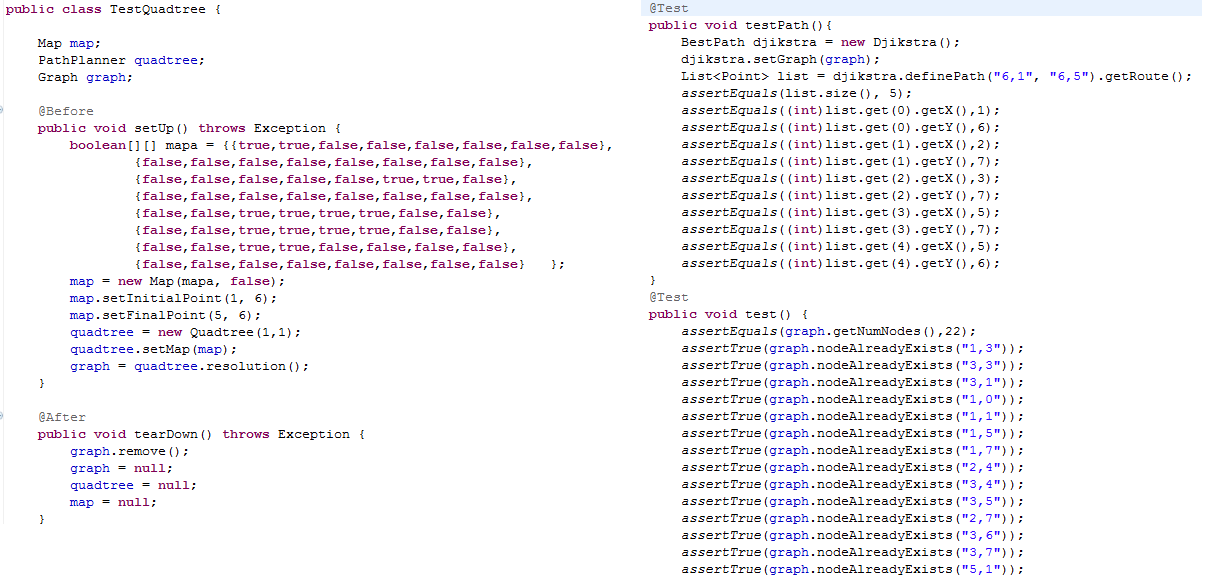
\includegraphics[keepaspectratio=true,scale=0.6]{figuras/testeinicial.png}
	\caption{teste inicial do \textit{framework}}
\end{figure}

\section{Testes de desempenho}

Após a validação do tema e verificado o funcionamento correto do fluxo de trabalho do \textit{framework}, o próximo passo foi o teste de desempenho do mesmo. Foi analizado o consumo de memória e o tempo de processamento para a avaliação do mesmo. 

Os testes foram realizado na IDE Netbeans, usando sua ferramenta de perfis. Esta ferramenta permite avaliar a memória que a JVM (Java Virtual Machine) está consumindo e o tempo de processamento de um programa, analizando cada método e classe. Ela fornece o número de vezes que um método é chamado, o tempo total deles, o tempo gasto por toda a classe e a porcentagem de cada um.

O algoritmo utilizado nestes testes foram o Quadtree. Este algoritmo permitiu uma análise mais rigorosa devido a sua implementação exigir maior memória para sua execução, através de sua recursão e de aumentar muito o número de objetos de acordo com o número e disposição dos obstáculos. Assim, foi analisado o \textit{framework} em seu pior caso, com mapas grandes, muitos obstáculos e com um algoritmo que cresce seu consumo junto com estas variantes.

\subsection{Testes de stress - simulação}

Os primeiros testes foram para testar os limites de processamento do Lego NXT, inserindo um mapa de 100 por 100 células e com uma enorme quantidade de obstáculos. Foi inserido 1089 obstáculos (uma a cada três casas) de 2 por 2 células. Dificilmente um ambiente assim seria utilizado para uso real, porém este teste visava apenas avaliar o quanto o hardware do robô utilizado suportava. As imagens 35 e 36 mostram o resultado da análise de processamento deste teste.

\begin{figure}[h]
	\centering
	\label{fig35}
		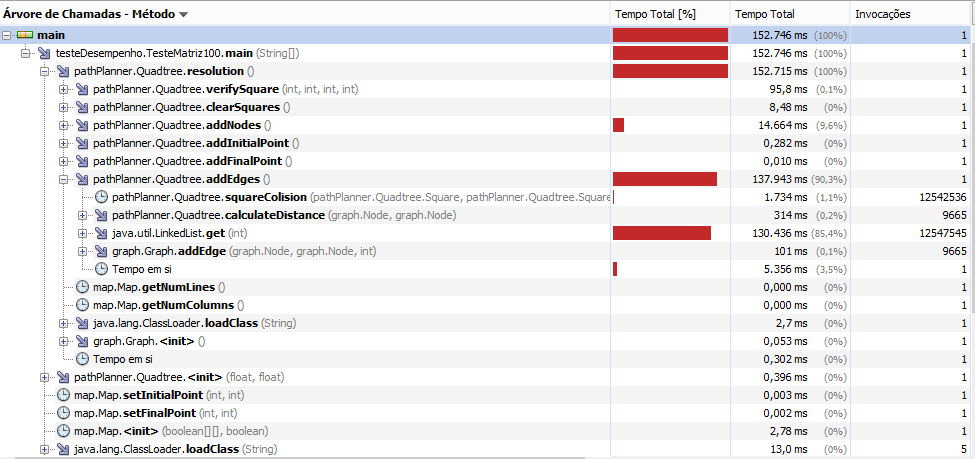
\includegraphics[keepaspectratio=true,scale=0.6]{figuras/teste100_1.PNG}
	\caption{teste de stress, tempo de execução}
\end{figure}

\begin{figure}[h]
	\centering
	\label{fig36}
		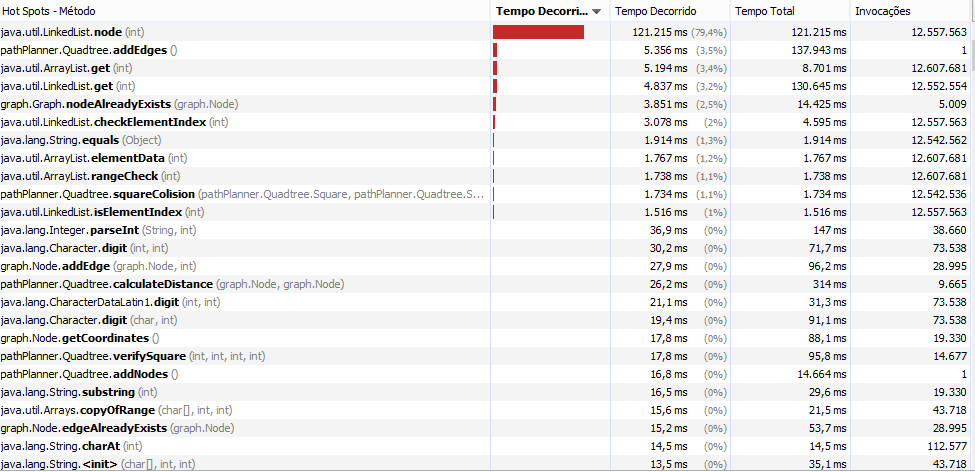
\includegraphics[keepaspectratio=true,scale=0.6]{figuras/teste100_2.PNG}
	\caption{teste de stress, métodos que mais foram utilizados}
\end{figure}

O teste levou ao todo quase 4 minutos para ser executado no computador, sendo este tempo repartido entre todos os processos da máquina e entre os vários processos dentro da própria máquina virtual Java. A análise retornou que o tempo gasto pelo \textit{framework} foi pouco mais de 152 milissegundos. A quantidade de tempo massiva gasta foi no método addEdges do Quadtree (90,3\%), aonde 85,4\% do tempo total foi com o método \textit{get} do LinkedList e apenas 3,5\% do tempo foi com o método em si.

A figura 36 nos mostra que, neste mesmo teste, a classe LinkedList consumiu muito mais tempo de processador que as classes do próprio \textit{framework}. Ao total, a classe foi responsável por 85,5\% do tempo de processamento.

Com relação ao gasto de memória, a função que mais consumiu foi a classe Square, do Quadtree. Justamente pela imensa quantidade de obstáculos e o pouco espaço entre eles, o algoritmo gerou uma imensa quantidade de quadrados para a geração do grafo, consumindo boa parte da memória. Não foi possível determinar a quantidade exata de memória gasta, pois a ferramenta inidicava o gasto total da máquina virtual Java e não apenas o do processo estudado.

Um segundo teste foi realizado com o mesmo ambiente e os resultados foram os mesmos, com poucas mudanças em relação ao tempo.

\subsection{Testes de stress no robô}

Ao embarcar este código no robô foi dado erro por falta de memória. O tamanho do mapa foi diminuído para 30 por 30, mantendo a mesma proporção de obstáculos e o espaçamento entre eles. Mesmo com esta diminuição ainda faltou memória no robô, precisando diminuir para 20 o tamanho do mapa. Foi medido com cronômetro digital que o tempo levado pelo \textit{framework} para calcular a trajetória com o mapa de 20x20 no robô foi de 15 segundos. Este mapa gerou um grafo com 500 nós e 1889 arestas. Este valor sozinho não pode definir o tamanho máximo de um grafo que o robô suporta (em um teste futuro um mapa com grafo menor não executou), pois o tamanho do mapa e outras estrutras também ocupam a memória e afetam o limite da máquina.

Apesar de dificilmente haver um ambiente onde haja tantos obstáculos ou que o robô só possa se mover em sobre uma grade, foi visto que mesmo com mapas pequenos a memória do Lego NXT não suporta o \textit{framework}. 

Outro teste feito no robô confirmou que o robô não suportaria o \textit{framework} para a maioria dos mapas. Nele, um mapa de 60x60 foi criado e inserido apenas 3 obstáculos. Este mapa foi retirado do simulador MRIT, que trabalha com um mapa de 60x60 e três obstáculos inicialmente. 

Ao embarcá-lo no Lego houve novamente estouro de memória. No grafo gerado por este mapa haviam 208 nós e 1060 arestas. O robô só conseguiu rodar o sistema ao retirar um dos obstáculos, gerando um grafo de 133 nós e 666 arestas. O tamanho do mapa foi mantido 60x60.

\subsection{Decisões tomadas}

Considerando que mesmo com mapas pequenos de 30x30 o Traveller pode não funcionar em alguns robôs e, principalmente, pelo teste com o mapa retirado do MRIT de 60x60 e 3 obstáculos não ter rodado no Lego, foi verificado que o consumo de memória do algoritmo Quadtree é muito alto e o \textit{framework} precisaria ser movido para fora do robô. Outros algoritmos como o Wavefront e Grafo de Visibilidade podem consumir bem menos memória, porém o \textit{framework} deve funcionar mesmo no pior caso, portanto a decisão de colocá-lo em um servidor foi tomada.

Vale lembrar que um mapa de 60x60 pode ainda ser pequeno dependendo da área de atuação do robô e do seu tamanho, já que a proporção entre robô e a área influencia no tamanho da matriz que o mesmo gerará.

Outra decisão foi a troca pela estrutura LinkedList pelo ArrayList. A grande maioria do tempo era gasto nesta classe, portanto ela foi substituída por outra semelhante também fornecida pelo Java. O ArrayList acessa um elemento com o método \textit{get} com ordem de complexidade O(1), enquanto o LinkedList faz o mesmo em ordem O(n). Mesmo o LinkedList apresentando vantagens quanto a gasto de memória e inserção e remoção de dados, essas funções eram pouco expressivas na totalidade do código, nem sequer chegando a aparecer nas estastísticas geradas, enquanto a função \textit{get} estava sempre entre as que mais consumiam tempo.

\section{Testes unitários e de sistema}

Para a realização dos testes foi utilizada a ferramenta JUnit, que fornece classes para a realização de testes unitários. Estas classes foram aproveitadas para realizar outros tipos de testes, como os testes de sistema explicados na seção 6.3.2.

A cada módulo construído e cada algoritmo implementado, uma nova suíte de testes eram desenvolvidas para validá-la. Os maiores detalhes sobre suas implementações são descritos nas seções a seguir.

\subsection{Testes unitários e cobertura de código}

Os testes unitários realizados buscavam a validação dos algoritmos, dos componentes e suas comunicações. Para tanto, foi realizado testes que chamavam as classes dos \textit{hot-spots} separadamente (sem se utilizar da controladora) para testar a saída de cada algoritmo.

Para os testes foram usados os mesmos mapas utilizados nos testes iniciais, que por seu tamanho reduzido permitiam calcular seus resultados manualmente para os quatro algoritmos e verificá-los com as funções do JUnit. Caso o algoritmo funcionasse nos casos testados era considerado correto.

Como a maioria dos métodos que executam a lógica são privados, foi verificado diretamente pelas funções do JUnit apenas as saídas dos algoritmos e se as mesmas eram totalmente compatíveis com os valores esperados. Caso as saídas fossem compatíveis em todos os casos, então os métodos internos estariam corretos.

Algumas funções do classe Map, de maior complexidade e relevãncia também foram diretamente testadas. Os métodos de expansão dos obstáculos e de localizar e retornar os vértices dos obstáculos também foram verificados pela suíte de testes pela sua importância nos algoritmos e possuírem uma lógica mais elaborada que as demais da mesa classe. Para a expansão foi expandido um obstáculo aonde o robô possuía o mesmo tamanho da célula da matriz (expanção de 1 célula), aonde o robô era menor (expansão também de 1 célula po arredondar para cima) e aonde o robô era 1,5 vezes maior (expansão de duas casas). Para a localização de vértices foi testado obstáculos retangulares, triangulares e hexagonais. Considerando que o mapa de é uma matriz, todo polígono pentagonal ou maior a vizinhança do ponto seria a mesma.

Além do JUnit, foi utilizado também o plugin Eclemma para a cobertuda de código. Este plugin é executado juntamente com os testes unitários e marca as linhas executas e qual a porcentagem do código foi verificada naquele teste. Como a execução do algoritmo executava todos os métodos internos as classes eram testadas e cobertas em sua maioria. Ao final de todos os testes, foi alcançado uma cobertura de código de XX\%.

\subsection{Testes de sistema e comparações com o simulador MRIT}

-comparação das simulações MRIT e framework
-comentar do 6º caso de teste q foi incluso só no final pra garantir que ñ da erro se ñ chegar a lugar algum

\section{Testes finais com o robô}

inserir a imagem codigofinal.PNG quando temrinar o código
fazer o voronoi e grafo de visib. e os teste unitarios e mrit 
bluecove (ver no site do lejos)
colocar a % da cobertura d ecódigo